\documentclass[aspectratio=169,9pt,dvipsnames]{beamer}
\usetheme{Boadilla}
% TODO! Replace Danish, France, FR, 10 centimes par litre, 100\euro{}, 160\euro{}

\usepackage{gensymb}
\usepackage[utf8]{inputenc}
\usepackage[english]{babel}
\usepackage[T1]{fontenc}

\usepackage{xcolor}
\usepackage{amsmath}
\usepackage{amsfonts}
\usepackage{amssymb}
\usepackage{graphicx}
\usepackage{changepage}
\usepackage{ragged2e}
\usepackage{amsmath,amssymb}
\usepackage{eurosym}
\usepackage{hyperref}
\usepackage{multicol}
\usepackage{caption}
\usepackage{subcaption}
\captionsetup{justification   = raggedright,
              singlelinecheck = false}
\usepackage[export]{adjustbox}

%\usepackage[toc,page]{appendix}
\usepackage{appendixnumberbeamer}
\usepackage{amssymb}% http://ctan.org/pkg/amssymb
\usepackage{pifont}% http://ctan.org/pkg/pifont
\newcommand{\cmark}{\ding{51}}%
\newcommand{\xmark}{\ding{55}}%

\usepackage{array,multirow,makecell}
\setcellgapes{1pt}
\makegapedcells
\newcolumntype{R}[1]{>{\raggedleft\arraybackslash }b{#1}}
\newcolumntype{L}[1]{>{\raggedright\arraybackslash }b{#1}}
\newcolumntype{C}[1]{>{\centering\arraybackslash }b{#1}}

\newcommand{\compresslist}{%
\setlength{\itemsep}{1pt}%
\setlength{\parskip}{0pt}%
\setlength{\parsep}{0pt}%
}

\beamertemplatenavigationsymbolsempty

\setbeamercolor{structure}{fg=teal}
\setbeamertemplate{itemize item}[circle]
\setbeamertemplate{section in toc}[square]
\setbeamertemplate{subsection in toc}[square]
\setbeamersize{text margin left=1cm, text margin right=1cm}
\setbeamertemplate{caption}[numbered]

\usepackage{lmodern}
\usefonttheme[onlymath]{serif}

\definecolor{teal_dark}{RGB}{26,140,140}



\justifying

\title[Climate survey - France]{\huge Climate survey - France}
\author[OECD]{OECD \\ \vspace{1cm}
    \textbf{Partial} sample of 1,691 respondents (instead of 2,000). \\ Results are reweighted along the gender, age, income, highest diploma, region and rural/urban dimensions.} % representative along the \\gender, age, income, region and rural/urban dimensions. \\ These variables define the quotas and the survey weights, used throughout.}% Representative along the \\gender, age, income, region and rural/urban dimensions but not representative along the education, ethnicity/race, vote and occupation dimensions. }
     % we don't use education, race nor vote as a quota, but it seems that highly educated and voters (and to a lesser extent, Biden voters) are over-represented, and Hispanic under-represented
%\author[Douenne \& \textbf{Fabre}]{\Large Thomas Douenne \& \textbf{Adrien Fabre} \large \\ $\quad$ \\ \textit{UvA (Amsterdam) \quad \textbf{ETH (Zurich)}}}
\date[\insertsection]{June 2021}





\begin{document}

	\begin{frame}

\titlepage
%\thispagestyle{empty}

	\end{frame}

	
\AtBeginPart{\frame{\partpage}}
\AtBeginSection[]
{
  \begin{frame}{Table of Contents}
  \begin{multicols}{2}
  \tableofcontents[currentsection]
  \end{multicols}
  \end{frame} 
}
\AtBeginSubsection[]
{
  \begin{frame}{Table of Contents}
  \begin{multicols}{2}
  \tableofcontents[currentsubsection]
  \end{multicols}
  \end{frame} 
}

\section{Summary}
%\begin{frame}{Project status}
%\begin{itemize}
%\item United States:
%	\begin{itemize}
%	\item 2,010 responses collected (focus of this presentation).
%	\end{itemize}
%\item France: 
%	\begin{itemize}
%	\item currently collecting answers
%	\end{itemize}
%\item  France: translation done
%
%\item India, UK, Spain, Germany:
%
%\begin{itemize}
%	\item Video script adjusted
%	\item Translation and video will start soon as we validate the questionnaire from the US experience
%\end{itemize}
%%Survey will be adjusted to the national context with input from colleagues.
%
%\end{itemize}
%\end{frame}

%\begin{frame}{Key findings}
%\begin{itemize}
%\item People worry about the negative impacts of climate change; Knowledge of climate change related impacts is relatively good.
%
%\item Most people agree that CC is a problem and that ambitious policies are needed.
%
%\item A majority under-estimate the necessary policy stringency to reduce emissions.
%
%\item Two-thirds are willing to change their behavior as long as it doesn’t affect their comfort and they have enough financial means (one-third is willing to forego some comfort).
%
%\item Support for our three specific policies is mixed, lower than in the pilot.
%
%\item The policy treatment increases public support for carbon tax and the ban on combustion-engine cars.
%\end{itemize}
%\end{frame} % TODO

\section{Socio-Demographics}
\begin{frame}{Education}%\addtocounter{framenumber}{-1}
    % \begin{itemize}
%\textbf{Education level:} Master degree should be 13\% to be representative. The rest is pretty much representative (population: 10\% without high school degree, 30\% only high school). % TODO
    %  \item \textbf{Ethnicity/Race:} Should be 60\% White, 19\% Hispanic, 13\% Black to be representative.
    % \end{itemize}
    \hspace{.2cm}
\begin{figure}[h!]
\centering
\caption{What is the highest level of education you have completed?}
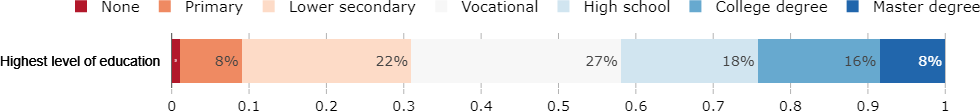
\includegraphics[width=.9\textwidth]{../figures/FR/education_FR.png} \\
\vspace{.3cm}
%\caption{What race or ethnicity do you identify with? (Multiple answers are possible)} % TODO
%\includegraphics[width=.5\textwidth]{../figures/FR/race_FR_comp.png}\\
\end{figure}
\end{frame}

% out
%\begin{frame}{Political affiliation}%\addtocounter{framenumber}{-1}
%    % \begin{itemize}
%    % \item \textbf{2020 election:} Should be 34\% Biden and 33\% Non-voter to be representative. 
%    % \end{itemize}
%\begin{figure}[h!] % TODO
%\centering
%\caption{Which candidate did you vote for in the last presidential election?}
%\includegraphics[width=.7\textwidth]{../figures/FR/vote_FR_comp.png} \\
%\end{figure}
%\end{frame}

\begin{frame}{Political affiliation}%\addtocounter{framenumber}{-1}
\begin{figure}[h!]
\centering
\caption{On economic policy matters, where do you see yourself on the liberal/conservative spectrum?}
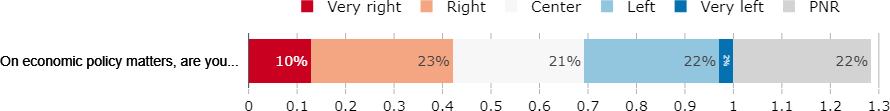
\includegraphics[width=\textwidth]{../figures/FR/left_right_FR.png} \\
\end{figure}
\end{frame}

\begin{frame}{Geography}%\addtocounter{framenumber}{-1}
\begin{figure}[h!]
\centering
\caption{Lives in an urban area (town > 20k people), retrieved from zipcode}
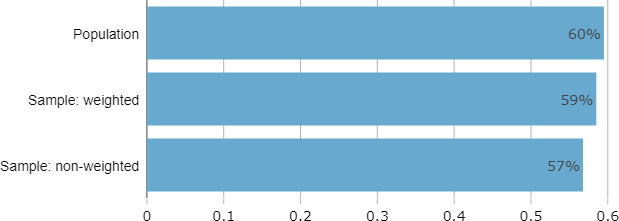
\includegraphics[width=.5\textwidth]{../figures/FR/urban_FR_comp.png} \\
\vspace{.2cm}
%\caption{Region, retrieved from zipcode} % TODO
%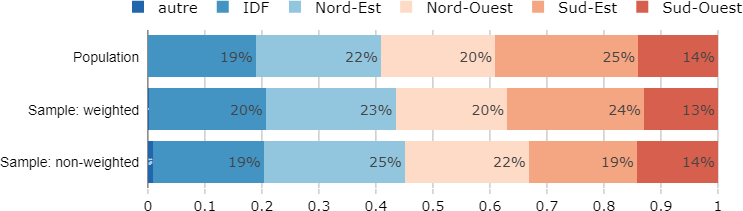
\includegraphics[width=.5\textwidth]{../figures/FR/region_FR_comp.png}
\end{figure}
\end{frame}

\begin{frame}{Gender and age}%\addtocounter{framenumber}{-1}
\begin{figure}[h!]
\centering
\caption{What is your gender?}
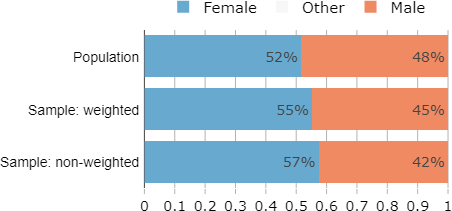
\includegraphics[width=.5\textwidth]{../figures/FR/gender_FR_comp.png} \\
\centering
\caption{How old are you?}
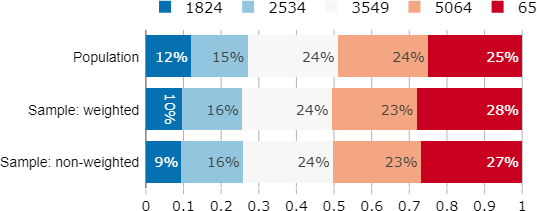
\includegraphics[width=.5\textwidth]{../figures/FR/age_FR_comp.png}
\end{figure}
\end{frame}

\begin{frame}{Income/wealth}%\addtocounter{framenumber}{-1}
\begin{figure}[h!]
\centering
\captionsetup{justification=centering}
\caption{What was the annual income of your household in 2019 (before withholding tax, for you and those who live with you)?}
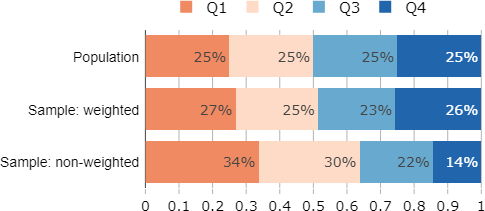
\includegraphics[width=.5\textwidth]{../figures/FR/income_FR_comp.png} \\
\vspace{.5cm}
\caption{\small What is the estimated value of your assets, or the assets of your household if you are married (in French dollars)? Include here all your possessions (home, car, savings, etc.) net of debt. For example, if you own a house worth \$300,000 and you have \$100,000 left to repay on your mortgage, your assets are \$200,000.}
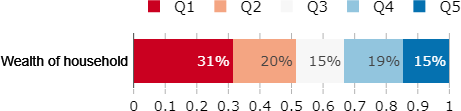
\includegraphics[width=.5\textwidth]{../figures/FR/wealth_FR.png} \\
\end{figure}
\end{frame}

\begin{frame}{Employment and hit by covid}%\addtocounter{framenumber}{-1}
\begin{figure}[h!]
\centering
\captionsetup{justification=centering}
\caption{What is your employment status?}
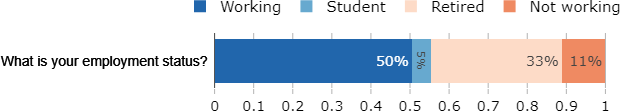
\includegraphics[width=.8\textwidth]{../figures/FR/employment_status_FR.png} \\
\vspace{.5cm}
% \caption{Which category best describes your main occupation (or last one if not currently employed)?}
% \includegraphics[width=.8\textwidth]{../figures/FR/occupation_FR.png} \\
\caption{Have you or a member of your household been laid off or had to take a cut in your salary or wages due to the COVID-19 pandemic?}
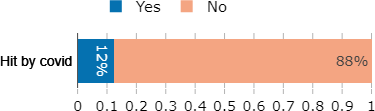
\includegraphics[width=.55\textwidth]{../figures/FR/hit_by_covid_FR.png}
\end{figure}
\end{frame}

% \begin{frame}{Hit by COVID-19}%\addtocounter{framenumber}{-1}
% \begin{figure}[h!]
% \centering
% \captionsetup{justification=centering}
% \caption{Have you or a member of your household been laid off or had to take a cut in your salary or wages due to the COVID-19 pandemic?}
% 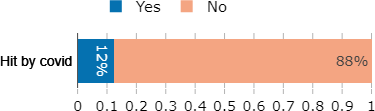
\includegraphics[width=.6\textwidth]{../figures/FR/hit_by_covid_FR.png} # TODO choose
% \end{figure}
% \end{frame}

\section{Political Views}

\begin{frame}{Interest in politics and environmental organizations}%\addtocounter{framenumber}{-1}
\vspace{-.5cm}
\begin{figure}[h!]
\caption{To what extent are you interested in politics?}
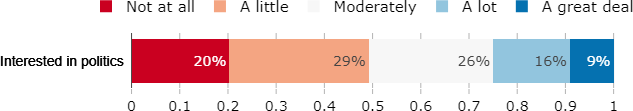
\includegraphics[width=.6\textwidth]{../figures/FR/interested_politics_FR.png} \\
%\caption{Could you trust the federal goverment to implement the following policies}
\vspace{.1cm}
\caption{Are you member of an environmental organization?}
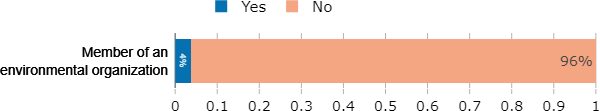
\includegraphics[width=.54\textwidth]{../figures/FR/member_environmental_orga_FR.png}\\
\vspace{.1cm}
\caption{Do you have any relatives who are environmentalists?}
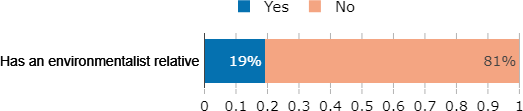
\includegraphics[width=.54\textwidth]{../figures/FR/relative_environmentalist_FR.png}\\
\end{figure}
\end{frame}

\begin{frame}{Presidential election vote}%\addtocounter{framenumber}{-1}
\vspace{-.5cm}
\begin{figure}[h!]
\caption{Did you vote in the 2020 French presidential election?}
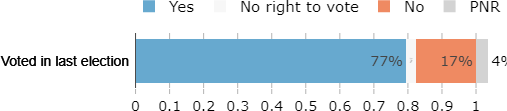
\includegraphics[width=.6\textwidth]{../figures/FR/vote_participation_FR.png} \\
%\caption{Could you trust the federal goverment to implement the following policies}
\vspace{.1cm}
\caption{Which candidate did you vote / would you have voted for in the last presidential election?}
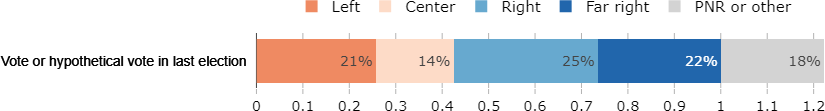
\includegraphics[width=.8\textwidth]{../figures/FR/vote_agg_FR.png} \\
% \caption{Which candidate did you vote for in the last presidential election?}
% \includegraphics[width=.6\textwidth]{../figures/FR/vote_all_FR.png} \\
% \caption{Did you vote in the 2016 French presidential election?}
% \includegraphics[width=.54\textwidth]{../figures/FR/vote_participation_2016_FR.png}\\
\end{figure}
\end{frame}

\begin{frame}{Political affiliation}%\addtocounter{framenumber}{-1}
\vspace{-.5cm}
\begin{figure}[h!]
\caption{On economic policy matters, where do you see yourself on the left/right spectrum?}
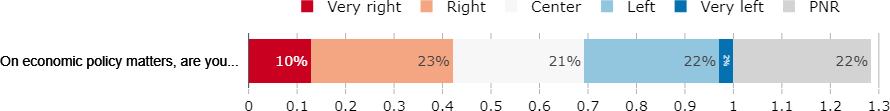
\includegraphics[width=.8\textwidth]{../figures/FR/left_right_FR.png} \\
%\caption{Could you trust the federal goverment to implement the following policies}
%\vspace{.1cm}
%\caption{What do you consider to be your political affiliation, as of today?}
%\includegraphics[width=.8\textwidth]{../figures/FR/political_affiliation_FR.png}\\
\end{figure}
\end{frame}


\section{Household Composition and Energy Characteristics}
\begin{frame}{}%\addtocounter{framenumber}{-1}
\begin{figure}[h!]
\caption{What is the main way you heat your home}

\centering
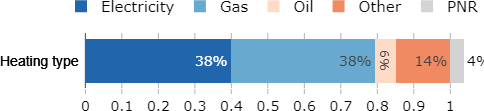
\includegraphics[width=.5\textwidth]{../figures/FR/heating_FR.png} \\
\vspace{.5cm}
\caption{In a typical month, how much do you spend on heating for your accommodation?}
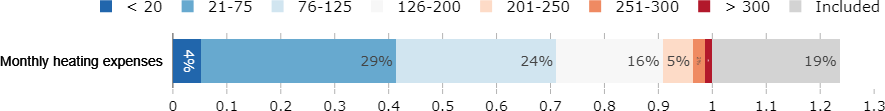
\includegraphics[width=.7\textwidth]{../figures/FR/heating_expenses_FR.png} \\
\vspace{.5cm}
\centering
\caption{How do you rate the insulation of your accommodation?}
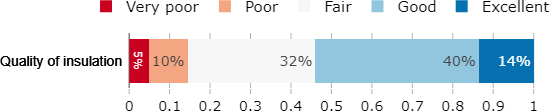
\includegraphics[width=.6\textwidth]{../figures/FR/insulation_FR.png}
\end{figure}
\end{frame}

\begin{frame}{}%\addtocounter{framenumber}{-1}
\begin{figure}[h!]
\centering
\caption{In a typical month, how much do you spend on gas for driving?}
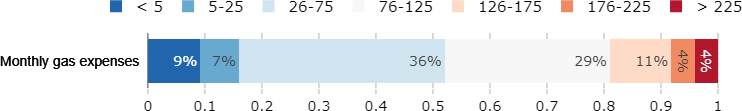
\includegraphics[width=.6\textwidth]{../figures/FR/gas_expenses_FR.png} \\
\vspace{.5cm}
\caption{How many round-trip flights did you take between 2017 and 2019?}
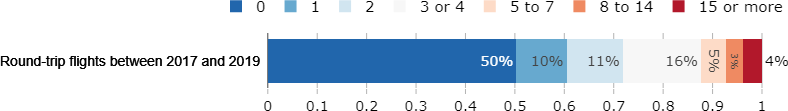
\includegraphics[width=.7\textwidth]{../figures/FR/flights_3y_FR.png}
\vspace{.5cm}
\caption{How often do you eat beef?}
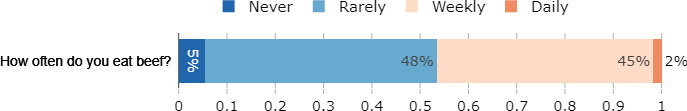
\includegraphics[width=.7\textwidth]{../figures/FR/frequency_beef_FR.png}
\end{figure}
\end{frame}

\begin{frame}{}%\addtocounter{framenumber}{-1}
\begin{figure}[h!]
\centering
\caption{Which mode of transport did you mainly use for each of the following trips in 2019?}
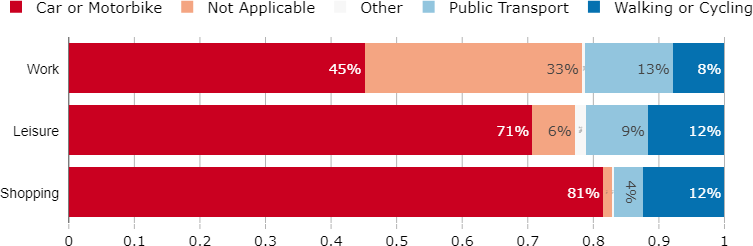
\includegraphics[width=.7\textwidth]{../figures/FR/transport_FR.png} \\
\vspace{.5cm}
\caption{How do you rate the availability (ease of access and frequency) of public transportation where you live?}
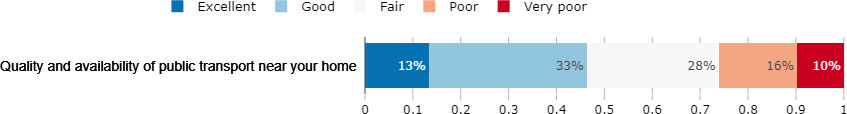
\includegraphics[width=.9\textwidth]{../figures/FR/availability_transport_FR.png}
\end{figure}
\end{frame}

\section{Essay}


\begin{frame}{}%\addtocounter{framenumber}{-1}
\begin{figure}[h!]
\centering
\caption{Word cloud -- When thinking about climate change, what are your main considerations? What should the French government do regarding climate change?
Please write as much as you would like, your response will be very useful.}
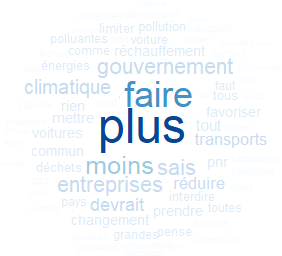
\includegraphics[width=.5\textwidth]{../figures/FR/CC_field_FR.png} \\
\end{figure}
\end{frame}

\section{Treatments}

% out
%\begin{frame}{Watched climate and/or policy videos attentively}%\addtocounter{framenumber}{-1} % TODO
%\begin{figure}[h!]
%\centering
%\caption{Number of wrong answers when answering knowledge questions about the content of the videos}
%\footnotesize \begin{itemize}
%\item What will be the rise in global average temperature in 2100 if greenhouse gas emissions continue on their current trend?
%\item In the absence of ambitious action against climate change, how frequent will extreme temperatures occur across the French by the end of the century?
%\item What is the emission limit described in the video? 
%\item How would a green infrastructure program be financed?
%\end{itemize}
%
%% \includegraphics[width=.7\textwidth]{../figures/FR/know_treatment.png}
%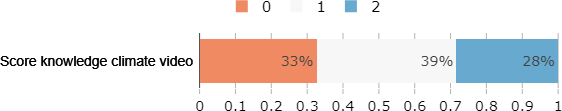
\includegraphics[width=.7\textwidth]{../figures/FR/know_treatment_climate_FR.png} \\
%\vspace{.5cm}
%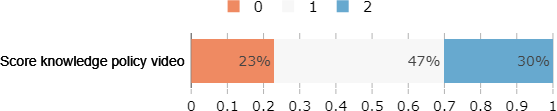
\includegraphics[width=.7\textwidth]{../figures/FR/know_treatment_policy_FR.png}
%\end{figure}
%\end{frame}


\section{Climate Knowledge}

%\begin{frame}{Climate knowledge: summary} % TODO
%    \begin{itemize}
%    \item People worry; knowledge is mixed.
%        \item In line with previous research, we find that about 60\% of Americans acknowledge that climate change exists and is anthropogenic.
%        \item A majority under-estimate the stringency of needed emission reductions. 
%        \item Most people understand what activities are most polluting, except for transport where knowledge is mixed. Most struggle identifying the correct ranking of regional per capita footprint.
%        \item Most people correctly understand that climate change will entail more natural disasters, but wrongly think that volcanic eruptions will be more frequent.
%        \item A majority thinks that CC puts humanity at risk of extinction, which is extremely pessimistic.
%        \item A relative majority thinks they will be personally affected by CC.
%    \end{itemize}
%\end{frame}

\begin{frame}{Climate change knowledge: general}%\addtocounter{framenumber}{-1}
\begin{figure}[h!]
\centering
\caption{How often do you think or talk with people about climate change?}
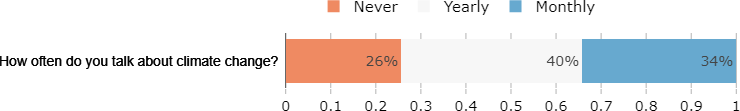
\includegraphics[width=.7\textwidth]{../figures/FR/CC_talks_FR.png}\\
\centering
% \caption{In your opinion, is climate change real?} \\
% 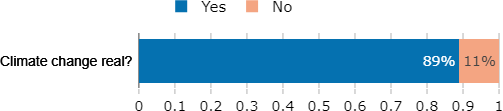
\includegraphics[width=.5\textwidth]{../figures/FR/CC_real_FR.png} \\
% \centering
% \caption{\textit{If answered yes to previous question:} What part of climate change do you think is due to human activity?}
% 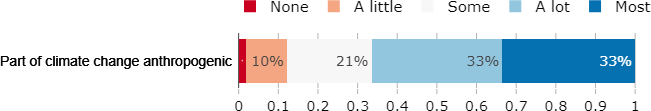
\includegraphics[width=.6\textwidth]{../figures/FR/CC_anthropogenic_non_deniers_FR.png} # TOOD choose
\caption{What part of climate change do you think is due to human activity?}
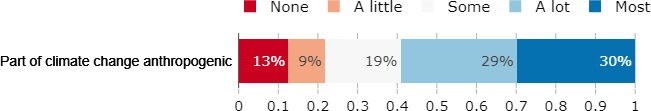
\includegraphics[width=.6\textwidth]{../figures/FR/CC_anthropogenic_FR.png}
\end{figure}
\end{frame}

\begin{frame}{Climate change knowledge: general}%\addtocounter{framenumber}{-1}
\begin{figure}[h!]
\centering
\caption{How knowledgeable do you consider yourself about climate change?}
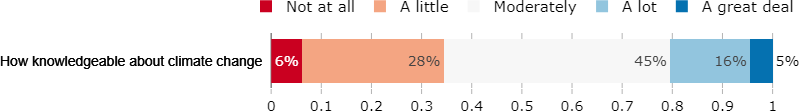
\includegraphics[width=.8\textwidth]{../figures/FR/CC_knowledgeable_FR.png}
\\
\centering
\caption{Do you agree or disagree with the following statement: ``Climate change is an important problem."}
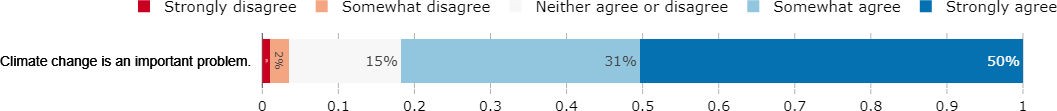
\includegraphics[width=.9\textwidth]{../figures/FR/CC_problem_FR.png}
\centering
\caption{Do you think that cutting global greenhouse gas emissions by half would be sufficient to eventually stop temperatures from rising? (Right answer: No)}
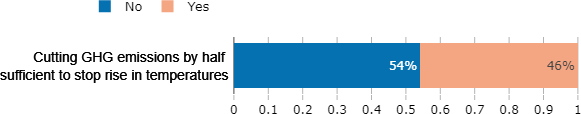
\includegraphics[width=.7\textwidth]{../figures/FR/CC_dynamic_FR.png}
\end{figure}
\end{frame}

\begin{frame}{Climate change knowledge: general}%\addtocounter{framenumber}{-1}
\begin{figure}[h!]
\centering
\caption{Which of the following elements contribute to climate change? (Multiple answers are possible)  }
\centering
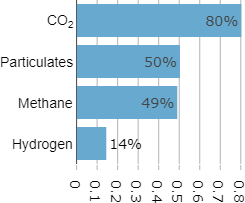
\includegraphics[width=.35\textwidth]{../figures/FR/GHG_FR.png}
\vspace{.2cm} \\
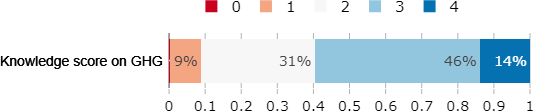
\includegraphics[width=.7\textwidth]{../figures/FR/score_GHG_FR.png}
\textit{Score on GHG = CO2 + methane + \textit{not} hydrogen + \textit{not}  particulates}
%\caption{Which of the following elements contribute to climate change? (Multiple answers are possible))}
\end{figure}
\end{frame}

% out
% \begin{frame}{Climate change knowledge: GHG footprints}%\addtocounter{framenumber}{-1}
% \begin{figure}[h!]
% \centering
% % \caption{Number of errors when ranking 3 items in terms of GHG emissions for three sectors}
% \caption{Kendall tau distance to correct ranking of GHG footprints for three sectors ($\sim$ number of mistakes)}
% 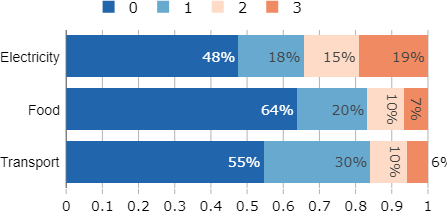
\includegraphics[width=.5\textwidth]{../figures/FR/scores_footprint_FR.png} \\
% \centering
% \caption{Rank the French/China/Western Europe/India in terms of GHG footprint}
% 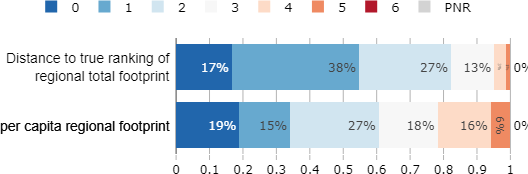
\includegraphics[width=.6\textwidth]{../figures/FR/score_footprint_regions_FR.png}
% \vspace{.2cm}
% % \\
% % \small{Correct ranking: plane>car>coach, beef>chicken>pasta, coal>gas>wind/ US>Western Europe>China>India} \\
% \end{figure}
% \end{frame}

\begin{frame}{Climate change knowledge}%\addtocounter{framenumber}{-1}
\begin{figure}[h!]
\centering
\caption{If a family of 4 travels 700 km from Copenhagen to Stockholm, with which mode of transportation do they emit the most greenhouse gases? % TODO!
Please rank the items from 1 (most) to 3 (least).}
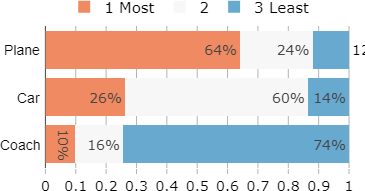
\includegraphics[width=.3\textwidth]{../figures/FR/footprint_transport_FR.png} \\
\centering
\caption{Which dish emits the most greenhouse gases? We consider that each dish weighs half a pound.
Please rank the items from 1 (most) to 3 (least).}
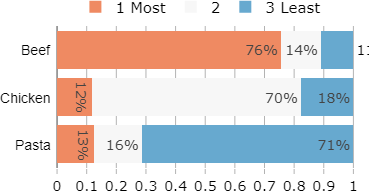
\includegraphics[width=.3\textwidth]{../figures/FR/footprint_food_FR.png}
\end{figure}
\end{frame}

\begin{frame}{Climate change knowledge}%\addtocounter{framenumber}{-1}
\begin{figure}[h!]
\centering
\caption{Which source of electric energy emits the most greenhouse gases to provide power for a house?}
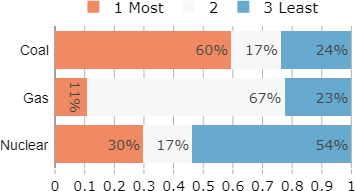
\includegraphics[width=.3\textwidth]{../figures/FR/footprint_elec_FR.png} \\
\end{figure}
\begin{figure}[h!]
\centering
\begin{subfigure}[b]{0.49\textwidth}
\centering
\caption{Which region contributes most to global greenhouse gas emissions?} % True ranking: China>US>EU>India. 
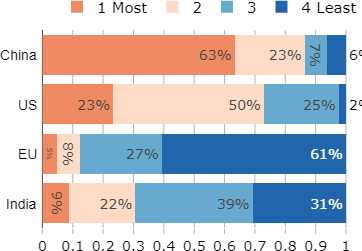
\includegraphics[width=.75\textwidth]{../figures/FR/footprint_region_no_miss_FR.png}
\end{subfigure}
\hfill
\begin{subfigure}[b]{0.49\textwidth}
\centering
\caption{In which region does the consumption of an average person contribute most to climate change?} % True ranking: US>EU>China>India. 
\includegraphics[width=.75\textwidth]{../figures/FR/footprint_pc_no_miss_FR.png}
\end{subfigure}
\end{figure}
\end{frame}

\begin{frame}{Impacts of climate change}%\addtocounter{framenumber}{-1}
\begin{figure}[h!]
\centering
%\caption{Impacts of climate change}
%\vspace{2mm}
\caption{If nothing is done to limit climate change, how likely do you think it is that climate change will lead to the following events?}
\includegraphics[width=.85\textwidth]{../figures/FR/CC_impacts_FR.png} \\
%\caption{}
\end{figure}
\end{frame}
% CC_dynamic

\section{Climate Attitudes}

%\begin{frame}{Climate attitudes: summary} % TODO
%    \begin{itemize}
%    \item Most people agree CC is a problem and ambitious policies are needed.
%    \item People are divided between optimistic and pessimistic (regarding future standards of living, technical feasibility to stop CC, and likelihood it will happen).
%    \item People are divided between those who foresee positive effects of climate policies and a third who foresees negative effects.
%    \item A third of people is willing to forego some comfort, two-thirds are willing to change behavior as long as it doesn't affect their comfort and they have enough financial means.
%    %   \item Only a slight majority recognizes that each of us are highly responsible for climate change, while around 70\% perceive companies are highly responsible for climate change.
%    %     \item People are divided about whether climate change can be halted by the end of the century, but only 20\% think ambitious policies are not important to halt it.
%    %     \item Around 20\% also think that ambitious policies would have strong negative effects on their lifestyle and around 30\% think ambitious policies would have negative effects on the French economy. 
%    %     \item It can be linked to the fact that only a minority is willing to adopt the most restrictive behaviors. Different types of constraints seem to influence their decisions.
%    \end{itemize}
%\end{frame}

\begin{frame}{Attitudes and risks}%\addtocounter{framenumber}{-1}
\begin{figure}[h!]
\centering
\caption{To what extent are the following groups responsible for climate change in France?}
\includegraphics[width=.8\textwidth]{../figures/FR/CC_responsible_FR.png}
\end{figure}
\end{frame}


\begin{frame}{Beliefs about the future}%\addtocounter{framenumber}{-1}
\begin{figure}[h!]
\caption{To what extent do you think that it is technically feasible to stop greenhouse gas emissions while maintaining satisfactory standards of living in France?}
\includegraphics[width=.6\textwidth]{../figures/FR/net_zero_feasible_FR.png} \\
\caption{To what extent do you think climate change already affects or will negatively affect your personal life?}
\includegraphics[width=.7\textwidth]{../figures/FR/CC_affects_self_FR.png} \\
% \caption{How ambitious do you think public policies should be to halt climate change?}
% \includegraphics[width=.7\textwidth]{../figures/FR/pro_ambitious_policies_FR.png}
\end{figure}
\end{frame}

\begin{frame}{Beliefs about ambitious climate policies}%\addtocounter{framenumber}{-1}
\begin{figure}[h!]
\centering
\caption{How likely is it that human kind halt climate change by the end of the century?}
\includegraphics[width=.7\textwidth]{../figures/FR/CC_will_end_FR.png}\\
\caption{If we decide to halt climate change through ambitious policies, to what extent do you think it would negatively affect your lifestyle?}
\includegraphics[width=.7\textwidth]{../figures/FR/effect_halt_CC_lifestyle_FR.png} \\
\caption{If we decide to halt climate change through ambitious policies, what would be the effects on the U.S economy and employment?}
\includegraphics[width=.7\textwidth]{../figures/FR/effect_halt_CC_economy_FR.png}
\end{figure}
\end{frame}

\begin{frame}{Willingness to change behaviors}%\addtocounter{framenumber}{-1}
\begin{figure}[h!]
\centering
\caption{Here are possible habits that experts say would help reduce greenhouse gas emissions.
To what extent would you be willing to adopt the following behaviors?}
\includegraphics[width=.8\textwidth]{../figures/FR/willing_FR.png} \\
\end{figure}
\end{frame}

% out
\begin{frame}{Factors needed to change lifestyle}%\addtocounter{framenumber}{-1}
\begin{figure}[h!]
\centering
\caption{How important are the factors below in order for you to adopt a sustainable lifestyle (i.e. limit driving, flying, and consumption, cycle more, etc.)?}
\includegraphics[width=1\textwidth]{../figures/FR/condition_FR.png}
\end{figure}
\end{frame}

%\begin{frame}{ }%\addtocounter{framenumber}{-1}
%\begin{figure}[h!]
%\centering
%\includegraphics[width=.6\textwidth]{../figures/FR/future_richness_FR.png}
%\end{figure}
%\end{frame}

\section{Policy 1: A ban on combustion-engine Cars}

\begin{frame}{Policy description}%\addtocounter{framenumber}{-1}
To fight climate change, car producers can be required by law to produce cars that emit less CO2 per mile of the cars they sell. The emission limit is lowered every year so that only electric or hydrogen vehicles can be sold after 2030. This policy is called a \textit{ban on combustion-engine cars}. 
\end{frame}


\begin{frame}{Effects of the policy}%\addtocounter{framenumber}{-1}

\begin{figure}[h!]
\centering
\caption{Do you agree or disagree with the following statements? A ban on combustion-engine cars would…}
\includegraphics[width=\textwidth]{../figures/FR/standard_effect_FR.png}
%\caption{}
\end{figure}
\end{frame}

\begin{frame}{Incidence}%\addtocounter{framenumber}{-1}
\begin{figure}[h!]
\centering
\caption{In your view, would the following groups win or lose if a ban on combustion-engine cars was implemented in France?}
\includegraphics[width=\textwidth]{../figures/FR/standard_win_lose_FR.png}
%\caption{}
\end{figure}
\end{frame}

\begin{frame}{Fairness and support}%\addtocounter{framenumber}{-1}
\begin{figure}[h!]
\centering
\caption{Do you agree or disagree with the following statement: ``A ban on combustion-engine cars is fair"?}
\includegraphics[width=\textwidth]{../figures/FR/standard_fair_FR.png}
\vspace{.5cm}
\centering
\caption{Do you support or oppose a ban on combustion-engine cars?}
\includegraphics[width=\textwidth]{../figures/FR/standard_support_FR.png}
\end{figure}

%\textbf{Support decreased} from 61\% in pilot, where it concerned ``an emission limit for cars''.
\end{frame}

\begin{frame}{}%\addtocounter{framenumber}{-1}
\begin{figure}[h!]
\centering
\caption{Do you support or oppose a ban on combustion-engine cars where alternatives such as public transports are made available to people?}
\includegraphics[width=\textwidth]{../figures/FR/standard_public_transport_support_FR.png}
%\caption{}
\end{figure}
\end{frame}

\section{Policy 2: Green Infrastructure Program}

\begin{frame}{Policy description}%\addtocounter{framenumber}{-1}
A green infrastructure program is a large public investment program, which would be financed by additional public debt, to accomplish the transition needed to cut greenhouse gases emissions. Investments would concern renewable power plants, public transportation, thermal renovation of building, and sustainable agriculture.
\end{frame}

\begin{frame}{Effects of the policy}%\addtocounter{framenumber}{-1}

%\textbf{Problem:} strong acquiescence bias. In the pilot, 57\% agreed that it was ``cost-effective''. Formulation changed to ``costly'' and 57\% agree.

\begin{figure}[h!]
\centering
\caption{Do you agree or disagree with the following statements? A green infrastructure program would…}
\includegraphics[width=\textwidth]{../figures/FR/investments_effect_FR.png}
%\caption{}
\end{figure}
\end{frame}

\begin{frame}{Incidence}%\addtocounter{framenumber}{-1}
\begin{figure}[h!]
\centering
\caption{In your view, would the following groups win or lose with a green infrastructure program?}
\includegraphics[width=\textwidth]{../figures/FR/investments_win_lose_FR.png}
%\caption{}
\end{figure}
\end{frame}

\begin{frame}{Fairness and support}%\addtocounter{framenumber}{-1}
\begin{figure}[h!]
\centering
\caption{Do you agree or disagree with the following statement: ``A green infrastructure program mainly financed by public debt is fair."}
\includegraphics[width=\textwidth]{../figures/FR/investments_fair_FR.png}
\vspace{.5cm}
\centering
\caption{Do you support or oppose a green infrastructure program?}
\includegraphics[width=\textwidth]{../figures/FR/investments_support_FR.png}
%\caption{}
\end{figure}


%\textbf{Support decreased} from 69\% in pilot.
\end{frame}

\begin{frame}{}%\addtocounter{framenumber}{-1}
\begin{figure}[h!]
\centering
\caption{Until now, we have considered that a green infrastructure program would be financed by public debt, but other sources of funding are possible.
What sources of funding do you find appropriate for a green infrastructure program? (Multiple answers are possible)}
\includegraphics[width=.8\textwidth]{../figures/FR/investments_funding_FR.png}
\end{figure}
\end{frame}

\section{Policy 3: Carbon Tax with Cash Transfers}

\begin{frame}{Policy description}%\addtocounter{framenumber}{-1}
To fight climate change, the French government can make greenhouse gas emissions costly, to make people and firms change their equipment and reduce their emissions. The government could do this through a policy called a carbon tax with cash transfers. Under such a policy, the government would tax all products that emit greenhouse gas. For example, the price of gasoline would increase by 10 centimes par litre. To compensate households for the price increases, the revenues from the carbon tax would be redistributed to all households, regardless of their income. Each adult would thus receive 160\euro{} per year.
\end{frame}

\begin{frame}{Effects of the policy}%\addtocounter{framenumber}{-1}
%
%\textbf{Problem:} strong acquiescence bias. In the pilot, 53\% agreed that it was ``cost-effective''. Formulation changed to ``costly'' and 57\% agree.

\begin{figure}[h!]
\centering
\caption{Do you agree or disagree with the following statements? A carbon tax with cash transfers would…}
\includegraphics[width=\textwidth]{../figures/FR/tax_transfers_effect_FR.png}
%\caption{}
\end{figure}
\end{frame}

\begin{frame}{Incidence}%\addtocounter{framenumber}{-1}
\begin{figure}[h!]
\centering
\caption{In your view, would the following groups win or lose under a carbon tax with cash transfers?}
\includegraphics[width=\textwidth]{../figures/FR/tax_transfers_win_lose_FR.png}
%\caption{}
\end{figure}
\end{frame}

\begin{frame}{Fairness and support}%\addtocounter{framenumber}{-1}
\begin{figure}[h!]
\centering
\caption{Do you agree or disagree with the following statement: ``A carbon tax with cash transfers is fair."}
\includegraphics[width=\textwidth]{../figures/FR/tax_transfers_fair_FR.png}
\vspace{.5cm}
\centering
\caption{Do you support or oppose a carbon tax with cash transfers?}
\includegraphics[width=\textwidth]{../figures/FR/tax_transfers_support_FR.png}
%\caption{}
\end{figure}

%\textbf{Support decreased} from 48\% in pilot, where it concerned ``an emission limit for cars''.
\end{frame}

\section{Comparison across the 3 Policies:}

\begin{frame}{Policy Incidence}%\addtocounter{framenumber}{-1}
\begin{figure}[h!]
\centering
\caption{\textit{Comparison of responses to each policy question:} Do you think that financially your household would win or lose from \textit{the policy}?}
\includegraphics[width=.7\textwidth]{../figures/FR/policies_win_lose_self_FR.png}
\vspace{-.1cm}
\centering
\caption{\textit{Comparison of responses to each policy question:} In your view, would those living in rural areas win or lose from \textit{the following policy}?}
\includegraphics[width=.7\textwidth]{../figures/FR/policies_win_lose_rural_FR.png}
%\caption{}
\end{figure}
\end{frame}

\begin{frame}{Policy Incidence}%\addtocounter{framenumber}{-1}
\begin{figure}[h!]
\centering
\caption{\textit{Comparison of responses to each policy question:} In your view, would high-income earners win or lose from \textit{the following policy}?}
\includegraphics[width=.7\textwidth]{../figures/FR/policies_win_lose_rich_FR.png}
\vspace{-.1cm}
\centering
\caption{\textit{Comparison of responses to each policy question:} In your view, would low-income earners win or lose from \textit{the following policy}?}
\includegraphics[width=.7\textwidth]{../figures/FR/policies_win_lose_poor_FR.png}
%\caption{}
\end{figure}
\end{frame}

\begin{frame}{Policy Incidence}%\addtocounter{framenumber}{-1}
\begin{figure}[h!]
\centering
\caption{\textit{Comparison of responses to each policy question:} In your view, would the middle-class win or lose from \textit{the following policy}?}
\includegraphics[width=.7\textwidth]{../figures/FR/policies_win_lose_middle_FR.png}
%\caption{}
\end{figure}
\end{frame}

\begin{frame}{Effects of the policy}%\addtocounter{framenumber}{-1}
\begin{figure}[h!]
\centering
\caption{\textit{Comparison of responses to each policy question:} Do you agree or disagree with the following statement? \textit{The policy} would have a large effect on the French economy and employment.}
\includegraphics[width=.9\textwidth]{../figures/FR/policies_large_effect_FR.png}
\vspace{-.1cm}
\centering
\caption{\textit{Comparison of responses to each policy question:} Do you agree or disagree with the following statement? \textit{The policy} would have a negative effect on the French economy and employment.}
\includegraphics[width=.9\textwidth]{../figures/FR/policies_negative_effect_FR.png}
%\caption{}
\end{figure}
\end{frame}

\begin{frame}{Effects of the policy}%
%\addtocounter{framenumber}{-1}

%\textbf{Problem:} strong acquiescence bias. In the pilot, 53-59\% agreed that it was ``cost-effective''. Formulation changed to ``costly'' and 56-57\% agree.
\begin{figure}[h!]
\vspace{-.1cm}
\centering
\caption{\textit{Comparison of responses to each policy question:} Do you agree or disagree with the following statement? \textit{The policy} would be costly to fight climate change}
\includegraphics[width=\textwidth]{../figures/FR/policies_cost_effective_FR.png}
%\caption{}
\end{figure}
\end{frame}


\begin{frame}{Fairness and support}%\addtocounter{framenumber}{-1}
\begin{figure}[h!]
\vspace{-.1cm}
\centering
\caption{\textit{Comparison of responses to each policy question:} Do you agree or disagree with the following statement:"The \textit{policy} is fair."}
\includegraphics[width=.8\textwidth]{../figures/FR/policies_fair_FR.png}
\vspace{-.1cm}
\centering
\caption{\textit{Comparison of responses to each policy question:} do you support or oppose \textit{the following policy}?}
\includegraphics[width=.8\textwidth]{../figures/FR/policies_support_FR.png}
%\caption{}
\end{figure}


%\textbf{Support decreased} from 48-61\% in pilot to 37-49\%. Largest drop for cars which was the most supported when it concerned ``an emission limit for cars'' .
\end{frame}

\section{Preferences for Climate Policies}

%\begin{frame}{Preferences for climate policies: summary}
%    \begin{itemize}
%       % \item Each specific policy proposed gathers a majority, the most favored being a ban on combustion-engine cars.
%        \item Each specific policy proposed gathers more support than opposition but the only one with more ``Strongly support'' than ``Strongly oppose'' is the green infrastructure program.
%        \item People are divided regarding the properties of these policies, and the answers may suffer from acquiescence or other bias. %although most think than a green infrastructure program and a ban on combustion-engine cars would be cost-effective to fight CC.
%        \item A majority supports each climate policy proposed (including coercive measures such as mandatory insulation of buildings) except tax policies and policies against meat. 
%        %\item The results regarding taxes go in the other direction than the first two pilots (maybe because of the more accurate level of taxes mentioned).
%        % \item However earmarking the revenues of the tax on fossil fuel, in particular for investments in green infrastructures or technologies, can lead a majority to support this policy.
%        \item Earmarking carbon tax revenues to green investments is the preferred option while uses of revenue for firms are the least favored.
%        \item A majority is willing to pay \$100/year to halt climate change, which is higher than the pilot' median at \$50/year (before we switched to binary question), but is still low. 
%        \item However, the median amount people are willing to donate to a charity is \$25 (over a potential gain of \$100). 
%        \item Most people are willing to insulate or replace heating of their accommodation, the cost of doing so is the bigger obstacle.
%        \end{itemize}
%\end{frame}



\begin{frame}{Other policies}%\addtocounter{framenumber}{-1}
\begin{figure}[h!]
\centering
\caption{Do you support or oppose the following climate policies?}
\vspace{2mm}
\includegraphics[width=\textwidth]{../figures/FR/policy_FR.png}
%\caption{}
\end{figure}
\end{frame}

\begin{frame}{Revenue recycling of carbon tax}%\addtocounter{framenumber}{-1}
\begin{figure}[h!]
\centering
\caption{Governments can use the revenues from carbon taxes in different ways. Would you support or oppose introducing a carbon tax that would raise gasoline prices by 10 centimes par litre, if the government used this revenue to finance...}
\vspace{2mm}
\includegraphics[width=\textwidth]{../figures/FR/tax_FR.png}
%\caption{}
\end{figure}
\end{frame}

\section{Willingness to Pay}

\begin{frame}{WTP}%\addtocounter{framenumber}{-1}
\begin{figure}[h!]
\centering
%\caption{Hoannually through an additional individual contribution to limit global warming to safe levels (less than 3.6 degrees Fahrenheit)?}
\caption{To fight global warming, the French government could implement a policy package to reduce emissions, for example by investing in clean technologies (renewable energy, electric vehicles, public transport, more efficient insulation, etc.). \\
The funding for these investments could be collected annually through an additional individual contribution for the foreseeable future. Assume that everyone in France as well as citizens of other countries would be required to contribute according to their means. \\ Are you willing to pay [amount] annually through an additional individual contribution to limit global warming to safe levels (less than 2 \degree{}C)?}
\includegraphics[width=.7\textwidth]{../figures/FR/wtp_FR.png} % TODO! scale. TODO: wtp_FR_anthropogenic?
\end{figure}
\end{frame}

\begin{frame}{Donation}
\begin{figure}[h!]
\centering
\caption{By taking this survey, you are entered into a lottery to win 100\euro{} (100\$). You can also donate a part of this additional compensation (should you be selected in the lottery) to a reforestation project through the charity The Gold Standard. If you win the 100\euro{} lottery, how much will you donate to the Gold Standard charity?}
\includegraphics[width=.9\textwidth]{../figures/FR/donation_agg_FR.png}
\end{figure}
%\textbf{We have a winner} who decided to donate the \$100 prize.
\end{frame}

\section{International Burden-Sharing}

%\begin{frame}{International burden-sharing: summary} % TODO
%    \begin{itemize}
%        \item The majority thinks that the French should do more whether other countries do more or less.
%        \item The favored burden sharing is the polluter-pays principle, although principles attributing a higher burden on high-income countries receive a relative majority support.
%        \item A solid majority supports global policies, in particular a global democratic assembly on CC, and a global tax on millionaires to finance low-income countries that comply with international standards regarding climate action.
%    \end{itemize}
%\end{frame}

\begin{frame}{Governance of climate policies}%\addtocounter{framenumber}{-1}
\vspace{-1cm}
\begin{figure}[h!]
\centering
\caption{\small{At which level(s) do you think public policies to tackle climate change need to be put in place? (Multiple answers are possible)}}
\includegraphics[width=.5\textwidth]{../figures/FR/scale_FR.png}
\end{figure}
\end{frame}

% out
\begin{frame}{US climate policy}%\addtocounter{framenumber}{-1}
\begin{figure}[h!]
\centering
\caption{Do you agree or disagree with the following statement: ``France should take measures to fight climate change."}
\includegraphics[width=1\textwidth]{../figures/FR/should_fight_CC_FR.png} \\
\vspace{1cm}
\caption{How should French climate policies depend on what other countries do?}
\includegraphics[width=1\textwidth]{../figures/FR/if_other_do_FR.png} \\
\end{figure}
\end{frame}


\begin{frame}{Burden-sharing}%\addtocounter{framenumber}{-1}
\begin{figure}[h!]
\centering
\caption{To achieve a given reduction of greenhouse gas emissions globally, costly investments are needed.
Ideally, how should countries bear the costs of fighting climate change?}
\vspace{2mm}
\includegraphics[width=\textwidth]{../figures/FR/burden_sharing_FR.png}
%\caption{}
\end{figure}
\end{frame}

\begin{frame}{Global policies}%\addtocounter{framenumber}{-1}
\begin{figure}[h!]
\centering
\caption{Do you support or oppose the following policies?}
\vspace{2mm}
\includegraphics[width=\textwidth]{../figures/FR/global_policies_FR.png}
%\caption{}
\end{figure}
\end{frame}

\section{Housing/Preferences for Bans vs. Incentives}

% out
\begin{frame}{Insulation}%\addtocounter{framenumber}{-1}
\vspace{-.5cm}
\begin{figure}[h!]
\caption{How likely is it that you will improve the insulation or replace the heating system of your accommodation over the next 5 years?}
\includegraphics[width=.6\textwidth]{../figures/FR/will_insulate_FR.png} \\
%\caption{Could you trust the federal goverment to implement the following policies}
\vspace{.1cm}
\caption{What are the main hurdles preventing you from improving the insulation or replace the heating system of your accommodation? (Multiple answers are possible)}
\includegraphics[width=.54\textwidth]{../figures/FR/obstacles_insulation_FR.png}\\
\end{figure}
\end{frame}

\begin{frame}{Insulation}%\addtocounter{framenumber}{-1}
\vspace{-.5cm}
\begin{figure}[h!]
%\caption{\textit{i)} To reduce fuel consumption for heating and cooling, the French government could subsidize half of the costs to renovate the insulation of residential buildings to meet a certain energy efficiency standard. \\
%\textit{ii)} Imagine that the French government makes it mandatory for all residential buildings to have insulation that meets a certain energy efficiency standard before 2040. The government would subsidize half of the insulation costs to help households with the transition. \\
%Do you support or oppose such a policy?}
\caption{Imagine that the French government makes it mandatory for all residential buildings to have insulation that meets a certain energy efficiency standard before 2040. The government would subsidize half of the insulation costs to help households with the transition. \\
Displayed in disruption variant: [Insulating your home can take long, may cause disruptions to your daily life during the renovation works, and may even require you to leave your home until the renovation is completed.]  \\
Do you support or oppose such policy? }
\includegraphics[width=.9\textwidth]{../figures/FR/insulation_support_variant_FR.png} 
% \vspace{.5cm}
% \includegraphics[width=.64\textwidth]{../figures/FR/ban_incentives_FR.png}
\end{figure}
\end{frame}

\begin{frame}{Cattle products}%\addtocounter{framenumber}{-1}
\vspace{-.5cm}
\begin{figure}[h!]
\caption{Imagine that, in order to fight climate change, the French government decides to limit the consumption of cattle products like beef and dairy.
Do you support or oppose the following options?}
\includegraphics[width=1\textwidth]{../figures/FR/beef_FR.png} 
% \vspace{.5cm}
% \includegraphics[width=.64\textwidth]{../figures/FR/ban_incentives_FR.png}
\end{figure}
\end{frame}

\section{Trust and institutions}

\begin{frame}{Trust}%\addtocounter{framenumber}{-1}
\vspace{-.5cm}
\begin{figure}[h!]
\caption{Do you agree or disagree with the following statement: ``Most people can be trusted."}
\includegraphics[width=.8\textwidth]{../figures/FR/can_trust_people_FR.png} \\
%\caption{Could you trust the federal goverment to implement the following policies}
\vspace{.1cm}
\caption{Do you agree or disagree with the following statement: ``Over the last decade the French government could generally be trusted to do what is right."}
\includegraphics[width=.8\textwidth]{../figures/FR/can_trust_govt_FR.png}\\
\end{figure}
\end{frame}

\begin{frame}{Perception of institutions, inequality, and the future}%\addtocounter{framenumber}{-1}
\vspace{-.2cm}
\begin{figure}[h!]
\caption{Some people think the government is trying to do too many things that should be left to individuals and businesses. Others think that government should do more to solve our country's problems.
Which come closer to your own view? }
\includegraphics[width=.7\textwidth]{../figures/FR/view_govt_FR.png} \\
%\caption{Could you trust the federal goverment to implement the following policies}
\vspace{.1cm}
\caption{How big of an issue do you think income inequality is in France?}
\includegraphics[width=.7\textwidth]{../figures/FR/problem_inequality_FR.png}\\
\vspace{.1cm}
\caption{Do you think that overall people in the world will be richer or poorer in 100 years from now?}
\includegraphics[width=.7\textwidth]{../figures/FR/future_richness_FR.png}
\end{figure}
\end{frame}


\section{Feedback}
\begin{frame}{Feedback on the survey}%\addtocounter{framenumber}{-1}
\vspace{-.2cm}
\begin{figure}[h!]
\caption{Do you feel that this survey was politically biased?}
\includegraphics[width=.6\textwidth]{../figures/FR/survey_biased_FR.png} \\
\vspace{.5cm}
\caption{The survey is nearing completion. You can now enter any comments, thoughts or suggestions in the field below.}
\includegraphics[width=.3\textwidth]{../figures/FR/comment_field_FR.png}
\end{figure}
\end{frame}

\section{Heterogeneity Analysis}

%\subsection{Republican vs. Democrat} % TODO
%\begin{frame}{Willingness to change behavior}%\addtocounter{framenumber}{-1}
%\vspace{-.2cm}
%\begin{figure}[h!]
%\caption{To what extent would you be willing to adopt the following behaviors? -– Limit Flying, by Political Affiliation}
%\includegraphics[width=.6\textwidth]{../figures/FR/willing_limit_flying_FR_pol.png} \\
%\vspace{.5cm}
%\caption{To what extent would you be willing to adopt the following behaviors? -- Limit Beef Consumption, by Political Affiliation}
%\includegraphics[width=.7\textwidth]{../figures/FR/willing_limit_beef_FR_pol.png} \\
%\end{figure}
%\end{frame}
%
%\begin{frame}{Perception}%\addtocounter{framenumber}{-1}
%\vspace{-.5cm}
%\begin{figure}[h!]
%\caption{Do you think that overall people in the world will be richer or poorer in 100 years from now? -– by Political Affiliation}
%\includegraphics[width=.7\textwidth]{../figures/FR/future_richness_FR_pol.png} \\
%\vspace{.5cm}
%\caption{If we decide to halt climate change through ambitious policies, to what extent do you think it would negatively affect your lifestyle? -- by Political Affiliation}
%\includegraphics[width=.7\textwidth]{../figures/FR/effect_halt_CC_lifestyle_FR_pol.png} \\
%\end{figure}
%\end{frame}
%
%\begin{frame}{Effects on own household}%\addtocounter{framenumber}{-1}
%\begin{figure}[h!]
%\caption{Do you think that financially your household would win or lose from the following policy? -- by Political Affiliation}
%\includegraphics[width=.6\textwidth]{../figures/FR/policies_win_lose_self_FR_pol.png} \\
%\vspace{.1cm}
%\caption{To what extent do you think climate change already affects or will negatively affect your personal life? -- by Political Affiliation}
%\includegraphics[width=.5\textwidth]{../figures/FR/CC_affects_self_FR_pol.png}
%\end{figure}
%\end{frame}
%
%\begin{frame}{Policies – support}%\addtocounter{framenumber}{-1}
%\vspace{-.5cm}
%\begin{figure}[h!]
%\caption{Do you support or oppose the following policy? -- by Political Affiliation}
%\includegraphics[width=.6\textwidth]{../figures/FR/policies_support_FR_pol.png} \\
%\vspace{.5cm}
%\caption{Do you support or oppose establishing a global democratic assembly whose role would be to draft international treaties against climate change? Each adult across the world would have one vote to elect members of the assembly. -- by Political Affiliation}
%\includegraphics[width=.6\textwidth]{../figures/FR/global_assembly_support_FR_pol.png} \\
%\end{figure}
%\end{frame}
%
%\begin{frame}{Policies – negative effects}%\addtocounter{framenumber}{-1}
%\vspace{-.5cm}
%\begin{figure}[h!]
%\caption{Do you agree or disagree with the following statement? This policy would have a negative effect on the French economy and employment -- by Political affiliation}
%\includegraphics[width=.8\textwidth]{../figures/FR/policies_negative_effect_FR_pol.png} \\
%\end{figure}
%\end{frame}

\subsection{Low-income vs. High-income}
\begin{frame}{Willingness to change behavior}%\addtocounter{framenumber}{-1}
\vspace{-.5cm}
\begin{figure}[h!]
\caption{To what extent would you be willing to adopt the following behaviors? -– Limit Flying, by Income}
\includegraphics[width=.6\textwidth]{../figures/FR/willing_limit_flying_FR_inc.png} \\
\vspace{.5cm}
\caption{To what extent would you be willing to adopt the following behaviors? -- Limit Beef Consumption, by Income}
\includegraphics[width=.7\textwidth]{../figures/FR/willing_limit_beef_FR_inc.png} \\
\end{figure}
\end{frame}

\begin{frame}{Perception}%\addtocounter{framenumber}{-1}
\vspace{-.5cm}
\begin{figure}[h!]
\caption{Do you think that overall people in the world will be richer or poorer in 100 years from now? -– by Income}
\includegraphics[width=.7\textwidth]{../figures/FR/future_richness_FR_inc.png} \\
\vspace{.5cm}
\caption{If we decide to halt climate change through ambitious policies, to what extent do you think it would negatively affect your lifestyle? -- by Income}
\includegraphics[width=.7\textwidth]{../figures/FR/effect_halt_CC_lifestyle_FR_inc.png} \\
\end{figure}
\end{frame}

\begin{frame}{Effects on own household}%\addtocounter{framenumber}{-1}
\begin{figure}[h!]
\caption{Do you think that financially your household would win or lose from the following policy? -- by Income}
\includegraphics[width=.6\textwidth]{../figures/FR/policies_win_lose_self_FR_inc.png} \\
\vspace{.1cm}
\caption{To what extent do you think climate change already affects or will negatively affect your personal life? -- by Income}
\includegraphics[width=.5\textwidth]{../figures/FR/CC_affects_self_FR_inc.png}
\end{figure}
\end{frame}

\begin{frame}{Policies – support}%\addtocounter{framenumber}{-1}
\vspace{-.5cm}
\begin{figure}[h!]
\caption{Do you support or oppose the following policy? -- by Income}
\includegraphics[width=.6\textwidth]{../figures/FR/policies_support_FR_inc.png} \\
\vspace{.5cm}
\caption{Do you support or oppose establishing a global democratic assembly whose role would be to draft international treaties against climate change? Each adult across the world would have one vote to elect members of the assembly. -- by Income}
\includegraphics[width=.6\textwidth]{../figures/FR/global_assembly_support_FR_inc.png} \\
\end{figure}
\end{frame}

\begin{frame}{Policies – negative effects}%\addtocounter{framenumber}{-1}
\vspace{-.5cm}
\begin{figure}[h!]
\caption{Do you agree or disagree with the following statement? This policy would have a negative effect on the French economy and employment -- by Income}
\includegraphics[width=.8\textwidth]{../figures/FR/policies_negative_effect_FR_inc.png} \\
\end{figure}
\end{frame}

\section{Treatment Effects}

%\begin{frame}{Treatment effects: summary} % TODO
%\begin{itemize}
%    \item When the treatments have almost no effect on general attitudes towards CC.
%   % \item In particular, all treatments are associated with the belief that CC can cause the extinction of human kind.
%    \item The Policy treatment has a large positive effect on support for a carbon tax with transfers (+13 p.p.), which can be linked to its effect on fairness and incidence on poor for this policy.
%    \item The Policy treatment also has a positive effect on support for the ban on combustion-engine (8 p.p.) and green infrastructure program (4 p.p.).
%    \item The Climate treatment has a negative effect on willingness to limit driving and support for green infrastructure program, which might be spurious correlation.
%    \item Low or null treatment effects may also be the result of respondents not updating the information on the policies (ban of combustion-engine cars and green infrastructure program), or due to lack of attentiveness to the videos (knowledge score on the videos seem low). 
%\end{itemize}
%\end{frame}

\begin{frame}{}%\addtocounter{framenumber}{-1}
\begin{table}[h!]
\caption{Attitudes towards Climate Change}
\begin{center}
\scalebox{.59}{
\begin{tabular}{@{\extracolsep{5pt}}lccccc} 
\\[-1.8ex]\hline 
\hline \\[-1.8ex] 
\\[-1.8ex] & CC caused by humans & CC likely to cause extinction & Donation (in \% of max) & FR should fight CC & Willing to limit driving \\ 
\hline \\[-1.8ex] 
 Control group mean & 0.567 & 0.587 & 24.924 & 0.778 & 0.321  \\ \hline \\[-1.8ex] Treatment: Climate & 0.096$^{***}$ & $-$0.034 & 2.490 & 0.006 & $-$0.020 \\ 
  & (0.029) & (0.031) & (1.694) & (0.026) & (0.029) \\ 
  & & & & & \\ 
 Treatment: Policy & 0.037 & $-$0.055$^{*}$ & $-$0.561 & $-$0.036 & $-$0.030 \\ 
  & (0.028) & (0.030) & (1.644) & (0.025) & (0.028) \\ 
  & & & & & \\ 
 Treatment: Both & 0.052$^{*}$ & $-$0.021 & $-$1.632 & $-$0.013 & 0.013 \\ 
  & (0.029) & (0.031) & (1.666) & (0.026) & (0.028) \\ 
  & & & & & \\ 
\hline \\[-1.8ex] 

Observations & 1,985 & 1,988 & 1,988 & 1,988 & 1,988 \\ 
\hline 
\hline \\[-1.8ex] 
\end{tabular} }
\end{center}
	{\tiny Note: The \textit{CC caused by humans} indicator variable equals one if the respondent thinks a lot or most of climate change is due to human actions. The \textit{CC likely to cause extinction} indicator variable equals one if the respondent thinks climate change is somewhat likely or very likely to cause the extinction of humankind if nothing is done to limit it. The \textit{Donation} variable is a continuous variable equal to the amount the respondent is willing to give to a charity. The \textit{Ambitious policies needed} indicator variable equals one if the respondent thinks policy must be a lot or a great deal ambitious in order to halt climate change. The \textit{Willing to limit driving} indicator variable equals one if the respondent is willing a lot or a great deal to limit driving. The three \textit{treatment} indicator variables indicate difference in mean compared to the control group (people who did not see any video). Controls include socio-demographic, economic affiliation, last vote and whether the respondent's household was hit by the COVID-19 pandemic. Standard errors are in parentheses.  *p$<$0.1; **p$<$0.05; ***p$<$0.01}
\end{table}
\end{frame}

\begin{frame}{}%\addtocounter{framenumber}{-1}
\begin{table}[h!]
\caption{Support for policies}
\begin{center}
\scalebox{.7}{
\begin{tabular}{@{\extracolsep{5pt}}lcccc} 
\\[-1.8ex]\hline 
\hline \\[-1.8ex] 
 & \multicolumn{4}{c}{Support} \\ 
\cline{2-5} 
\\[-1.8ex] & Carbon tax with transfers & Green Infrastructure Program & Ban on combustion-engine cars & Average over 3 policies \\ 
\hline \\[-1.8ex] 
 Control group mean & 0.282 & 0.582 & 0.274 & 0.444  \\ \hline \\[-1.8ex] Treatment: Climate & 0.061$^{**}$ & 0.037 & 0.032 & 0.035 \\ 
  & (0.030) & (0.030) & (0.029) & (0.031) \\ 
  & & & & \\ 
 Treatment: Policy & 0.079$^{***}$ & 0.033 & 0.061$^{**}$ & 0.051$^{*}$ \\ 
  & (0.029) & (0.029) & (0.028) & (0.030) \\ 
  & & & & \\ 
 Treatment: Both & 0.146$^{***}$ & 0.037 & 0.100$^{***}$ & 0.099$^{***}$ \\ 
  & (0.029) & (0.030) & (0.029) & (0.030) \\ 
  & & & & \\ 
\hline \\[-1.8ex] 

Observations & 1,988 & 1,988 & 1,988 & 1,988 \\ 
\hline 
\hline \\[-1.8ex] 
\end{tabular} }
\end{center}
	{\footnotesize Note: The dependent variables are indicator variables equal to one if the respondent `Strongly supports'' or ``Somewhat supports'' the policy. The \textit{Average over 3 policies} takes the average of the respondent's answers for the three policies. It equals one if the respondent support all three policies, $2/3$ if she supports two, $1/3$ if she support only one, and 0 if she supports none. See notes under previous Table for a description of the covariates.
	\newline Controls include socio-demographic, economic affiliation, last vote and whether the respondent's household was hit by the COVID-19 pandemic. Standard errors are in parentheses. *p$<$0.1; **p$<$0.05; ***p$<$0.01}
\end{table}
\end{frame}

\begin{frame}{}%\addtocounter{framenumber}{-1}
\begin{table}[h!]
\caption{Attitudes towards policies}
\begin{center}
\scalebox{.7}{
\begin{tabular}{@{\extracolsep{5pt}}lccccc} 
\\[-1.8ex]\hline 
\hline \\[-1.8ex] 
\\[-1.8ex] & Fair & HH would win & Poor would win & Large economic effect & Negative economic effect \\ 
\hline \\[-1.8ex] 
 Control group mean & 0.436 & 0.292 & 0.173 & 0.592 & 0.41  \\ \hline \\[-1.8ex] Treatment: Climate & 0.011 & 0.040 & 0.014 & 0.013 & 0.007 \\ 
  & (0.030) & (0.029) & (0.026) & (0.030) & (0.031) \\ 
  & & & & & \\ 
 Treatment: Policy & 0.025 & 0.026 & 0.091$^{***}$ & 0.035 & 0.017 \\ 
  & (0.030) & (0.029) & (0.026) & (0.030) & (0.031) \\ 
  & & & & & \\ 
 Treatment: Both & 0.091$^{***}$ & 0.094$^{***}$ & 0.149$^{***}$ & 0.053$^{*}$ & 0.028 \\ 
  & (0.031) & (0.030) & (0.026) & (0.031) & (0.031) \\ 
  & & & & & \\ 
\hline \\[-1.8ex] 

Observations & 1,982 & 1,864 & 1,963 & 1,982 & 1,982 \\ 
\hline 
\hline \\[-1.8ex] 
\end{tabular} }
\end{center}
	{\scriptsize Note: The dependent variables are discrete variables equal either to 0, $1/3$, $2/3$, or 1. They are equal to the average over the three policies mentioned in Table ``Support policies''. The \textit{Fair} variable equals one if the respondent strongly agrees or somewhat agrees that each of the three policies are fair. The \textit{HH/Poor would win} variables equal one if the respondent thinks her househould/the poorest would win a lot or mostly win from the three policies. The \textit{Large/Negative economic effect} variables equal one if the respondent strongly agrees or somewhat agrees that the three policies would have a large/negative impact on the French economy and employment. 
	\newline Controls include socio-demographic, economic affiliation, last vote and whether the respondent's household was hit by the COVID-19 pandemic. Standard errors are in parentheses. *p$<$0.1; **p$<$0.05; ***p$<$0.01}
\end{table}
\end{frame}

\section{Regressions Results and Political Heterogeneity}

\begin{frame}{Regression of Indexes}%\addtocounter{framenumber}{-1}
\vspace{-.5cm}
\begin{figure}[h!]
\caption{Coefficients from regressions}
\includegraphics[width=.5\textwidth]{../figures/FR/coef_indexes_FR.png} \\
\end{figure}
\end{frame}

\begin{frame}{Descriptions of Indexes}
\begin{itemize}
  \item Indexes are non-weighted average of z-scores
  \item Each z-score is normalizeed with survey weights, control mean group and sd mean group. Impute mean of treatment group to missing values.
  \item \textit{Affected Index:} polluting sector, transports used, expenses in gas and heating, availability of public transport, size of town, urbanity.
  \item \textit{Knowledge Index:} scores on footprint questions, knowledge on the dynamic, reality, and anthropogenic diemsnions of climate change, knowledge of the impacts origins of climate change.
  \item \textit{Knowledge Index (EFA):} weights are loadings from explanatory factor analysis.
\end{itemize}
\end{frame}

\begin{frame}{Regression of Support on Indexes}%\addtocounter{framenumber}{-1}
\vspace{-.5cm}
\begin{figure}[h!]
\caption{Coefficients from regressions}
\includegraphics[width=.5\textwidth]{../figures/FR/coef_support_indexes_FR.png} \\
\end{figure}
\end{frame}

\begin{frame}{Regression of Political Affiliation}%\addtocounter{framenumber}{-1}
\vspace{-.5cm}
\begin{figure}[h!]
\caption{Coefficients from regressions}
\includegraphics[width=.5\textwidth]{../figures/FR/coef_Right_FR.png} \\
\end{figure}
\end{frame}

\begin{frame}{Heterogeneity Analysis for Support -- Political Affiliation}%\addtocounter{framenumber}{-1}
\vspace{-.5cm}
\begin{figure}[h!]
\caption{Support by political affiliation}
\includegraphics[width=.5\textwidth]{../figures/FR/support_by_political_FR.png} \\
\end{figure}
\end{frame}

\end{document}
